\subsection{Убираем высокие частоты}

\def\num{1}
\def\a{3}
\def\from{-2}
\def\to{4}
\def\b{1}
\def\c{0}
\def\d{0}
\def\T{10}
\def\imageclip{10}

\subsubsection{Рассматриваемая функция}
Рассмотрим функцию $g(t)$ при параметрах $a=$~\a, $t1 =$~ \from, $t_2 =$~\to ~(см. рисунок~\ref{fig:wave_function_\num}) 
и ее \textit{зашумленную} версию $u(t)$ с параметрами $b =$~\b, $c =$~\c, $d =$~\d ~(см. рисунок~\ref{fig:noised_wave_function_\num}).
на промежутке $[-T/2,~T/2]$ с $T =$~\T.

\FloatBarrier
\subsubsection{Графики рассматриваемой и зашумленной функции}
\begin{figure}[ht!]
    \centering
    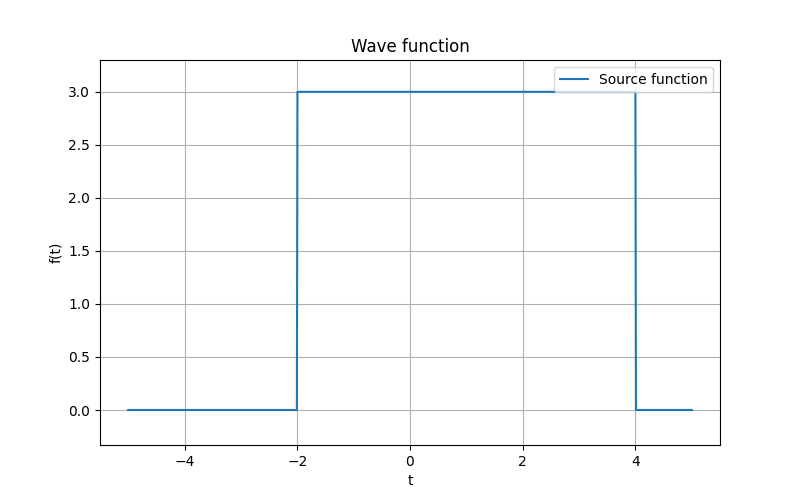
\includegraphics[width=\textwidth]{../results/\num/wave_function.png}
    \caption{Функция $g(t)$ с параметрами $a = \a$, $t_1 = \from$, $t_2 = \to$}
    \label{fig:wave_function_\num}
\end{figure}

\begin{figure}[ht!]
    \centering
    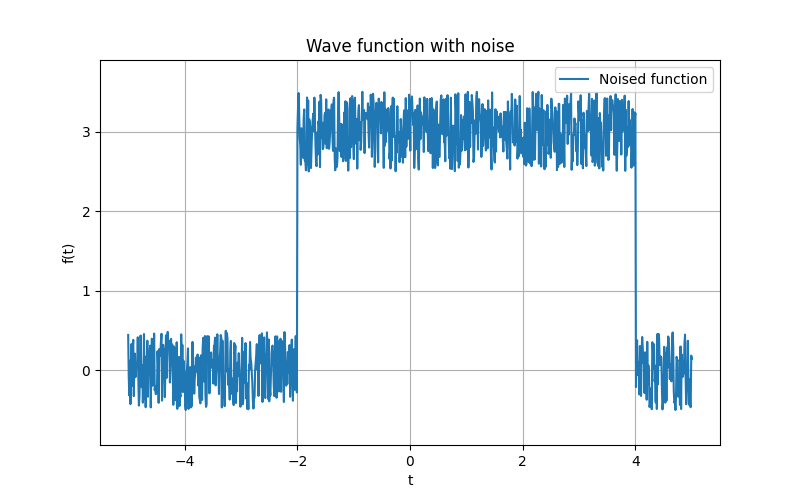
\includegraphics[width=\textwidth]{../results/\num/noised_wave_function.png}
    \caption{Функция $u(t)$ с параметрами $b = \b$, $c = \c$, $d = \d$}
    \label{fig:noised_wave_function_\num}
\end{figure}

\FloatBarrier
\subsubsection{Нахождение образов исходной и зашумленной функций}
Найдем образы исходной (см. рисунок~\ref{fig:wave_function_image_\num}) 
и зашумленной (см. рисуно~\ref{fig:noised_wave_function_image_\num}) функций с помощью преобразования Фурье. 

\begin{figure}[ht!]
    \centering
    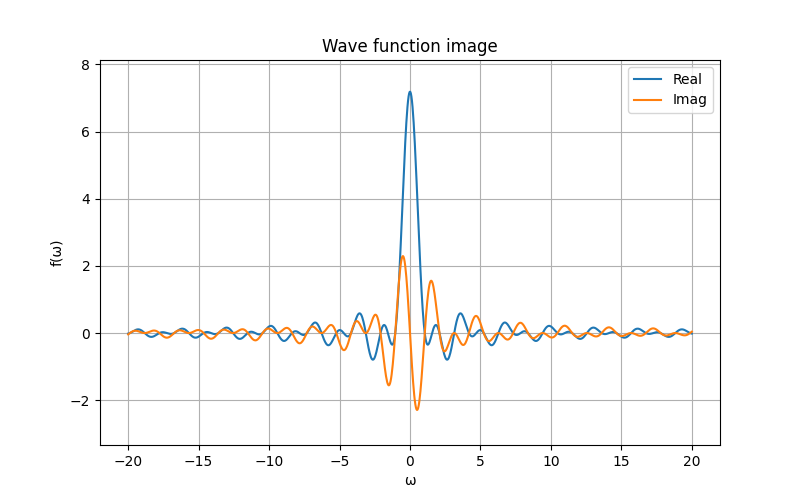
\includegraphics[width=\textwidth]{../results/\num/wave_function_image.png}
    \caption{Образ функция $g(t)$ с параметрами $a = \a$, $t_1 = \from$, $t_2 = \to$}
    \label{fig:wave_function_image_\num}
\end{figure}

\begin{figure}[ht!]
    \centering
    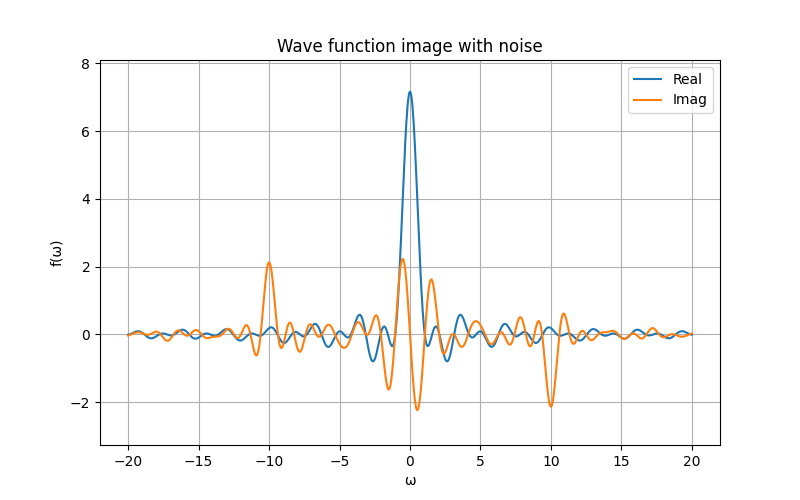
\includegraphics[width=\textwidth]{../results/\num/noised_wave_function_image.png}
    \caption{Образ функция $u(t)$ с параметрами $b = \b$, $c = \c$, $d = \d$}
    \label{fig:noised_wave_function_image_\num}
\end{figure}

Разница между образами исходной и зашумленной функций не заметна на графиках. 
Это может быть связано с тем, что высокочастотные компоненты функции $u(t)$ не сильно отличаются от нуля.

\FloatBarrier
\subsubsection{Фильтрация высоких частот}
\textit{Обрежем} образ функции $u(t)$, убрав компоненты, соответствущие высоким частотам (см. рисунок~\ref{fig:noised_wave_function_image_clipped_\num}).

\begin{figure}[ht!]
    \centering
    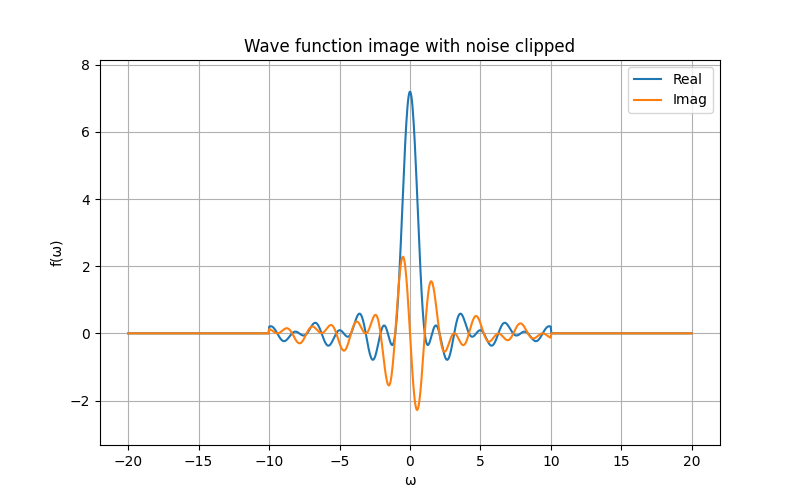
\includegraphics[width=\textwidth]{../results/\num/noised_wave_function_image_clipped.png}
    \caption{Обрезанный образ функция $u(t)$ при $\omega_0=$~\imageclip}
    \label{fig:noised_wave_function_image_clipped_\num}
\end{figure}

Как и ожидалось, высокочастотные компоненты ($|\omega| > \omega_0$) стали равны нулю. 
Теперь выполним обратное преобразование Фурье (используя обрезанный образ), получив при этом фильтрованную версию функции (см. рисунок~\ref{fig:wave_function_clipped_restored_\num}).

\begin{figure}[ht!]
    \centering
    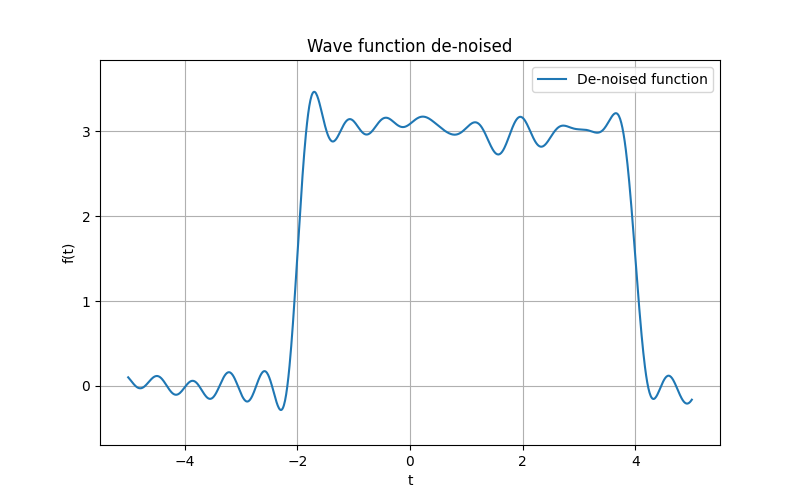
\includegraphics[width=\textwidth]{../results/\num/wave_function_clipped_restored.png}
    \caption{Фильтрованная функция $u(t)$ при $\omega_0=$~\imageclip}
    \label{fig:wave_function_clipped_restored_\num}
\end{figure}

Видим, что шумов стало меньше, но функция не идентична исходной, так как удаление высокочастотных компонент сказалось не только на шумах, но и на самой функции. 
Сравнительные графики исходной и фильтрованной функций представлены на рисунке~\ref{fig:wave_function_comparison_\num}. 
\begin{figure}[ht!]
    \centering
    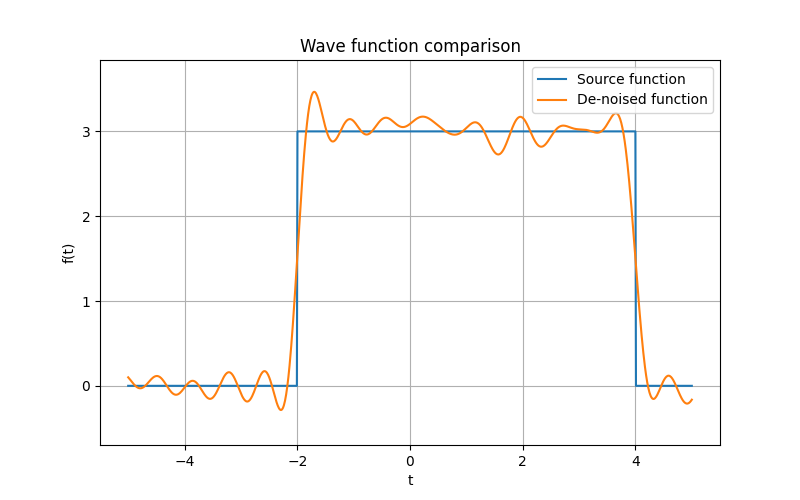
\includegraphics[width=\textwidth]{../results/\num/wave_function_comparison.png}
    \caption{Исходная и фильтрованная функция при $\omega_0=$~\imageclip}
    \label{fig:wave_function_comparison_\num}
\end{figure}

Таким образом, фильтрация высоких частот позволяет убрать шумы, не сильно влияя на саму функцию.

\FloatBarrier
\subsubsection{Сравнение модулей образов}
Сравним модули образов исходной и фильтрованной функций (см. рисунок~\ref{fig:wave_function_image_abs_\num}~и~\ref{fig:wave_function_clipped_restored_image_abs_\num}).

\begin{figure}[ht!]
    \centering
    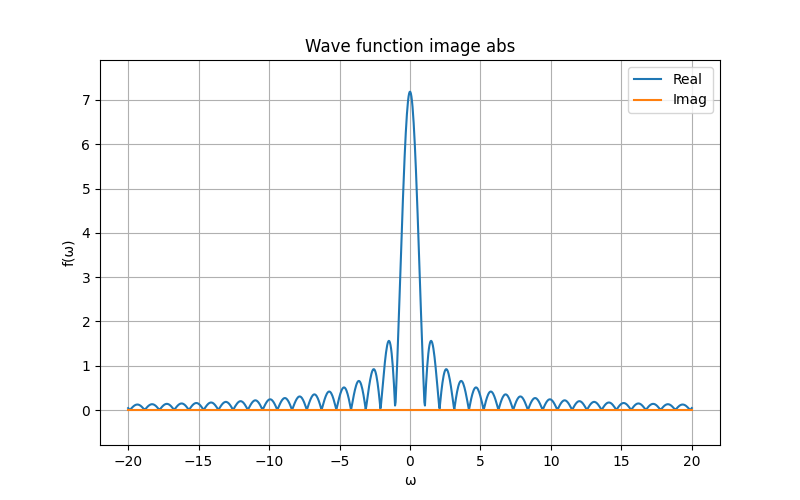
\includegraphics[width=\textwidth]{../results/\num/wave_function_image_abs.png}
    \caption{Модуль образа исходной функции $g(t)$}
    \label{fig:wave_function_image_abs_\num}
\end{figure}

\begin{figure}[ht!]
    \centering
    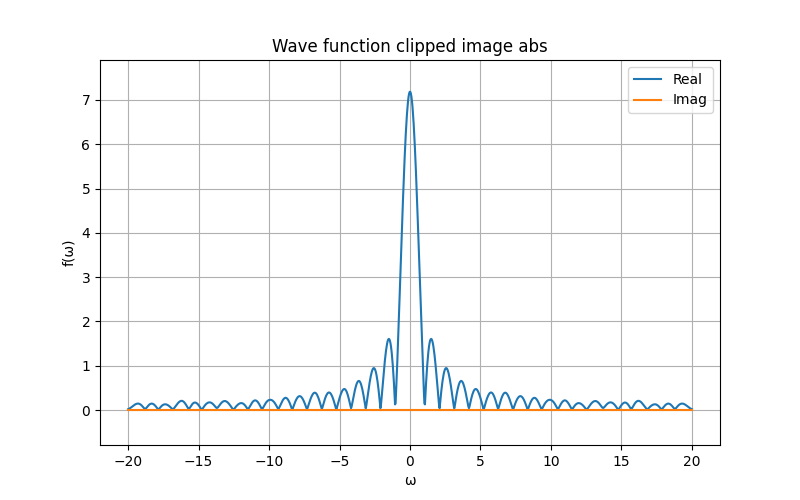
\includegraphics[width=\textwidth]{../results/\num/wave_function_clipped_restored_image_abs.png}
    \caption{Модуль образа фильтрованной функции $u(t)$ при $\omega_0=$~\imageclip}
    \label{fig:wave_function_clipped_restored_image_abs_\num}
\end{figure}

Видим, что практически частоты выше $\omega_0$ обнулились, при этом низкочастотные компоненты остались практически неизменными. 

\FloatBarrier
\subsubsection{Исследование влияния частоты среза на фильтрацию}

Рассмотрим несколько значений частоты среза $\omega_0$ при $b=$~\b~и сравним результаты фильтрации.

\def\num{2}
\def\imageclip{5}

% \begin{figure}[ht!]
%     \centering
%     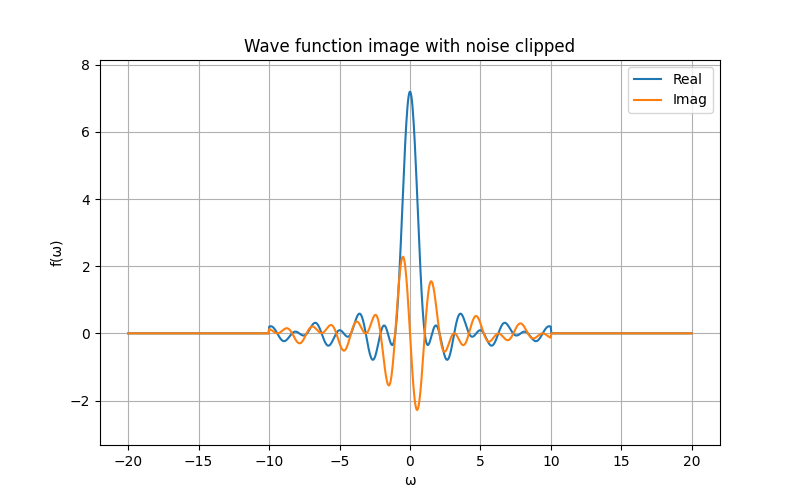
\includegraphics[width=\textwidth]{../results/\num/noised_wave_function_image_clipped.png}
%     \caption{Обрезанный образ функция $u(t)$ при $\omega_0=$~\imageclip}
%     \label{fig:noised_wave_function_image_clipped_\num}
% \end{figure}

\begin{figure}[ht!]
    \centering
    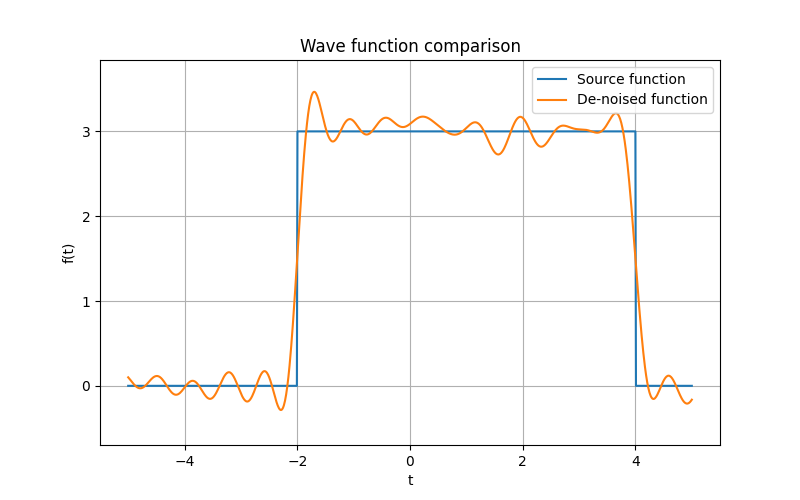
\includegraphics[width=\textwidth]{../results/\num/wave_function_comparison.png}
    \caption{Исходная и фильтрованная функция при $\omega_0=$~\imageclip}
    \label{fig:wave_function_comparison_\num}
\end{figure}


\def\num{3}
\def\imageclip{2}

% \begin{figure}[ht!]
%     \centering
%     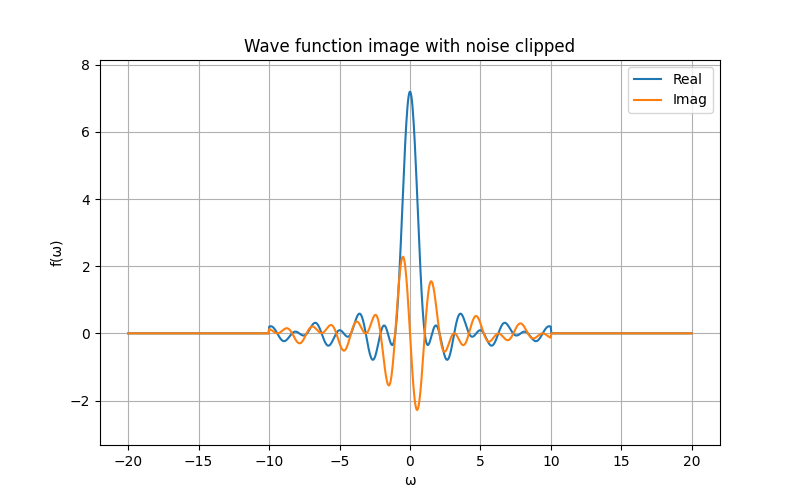
\includegraphics[width=\textwidth]{../results/\num/noised_wave_function_image_clipped.png}
%     \caption{Обрезанный образ функция $u(t)$ при $\omega_0=$~\imageclip}
%     \label{fig:noised_wave_function_image_clipped_\num}
% \end{figure}

\begin{figure}[ht!]
    \centering
    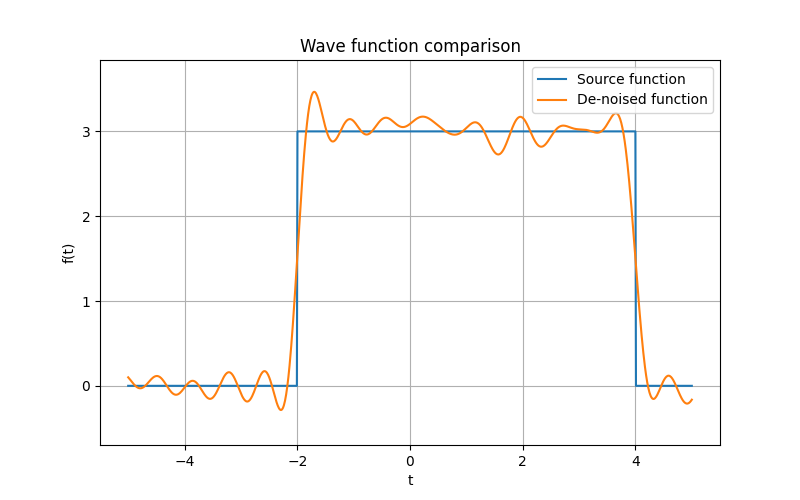
\includegraphics[width=\textwidth]{../results/\num/wave_function_comparison.png}
    \caption{Исходная и фильтрованная функция при $\omega_0=$~\imageclip}
    \label{fig:wave_function_comparison_\num}
\end{figure}

\def\num{4}
\def\imageclip{20}

% \begin{figure}[ht!]
%     \centering
%     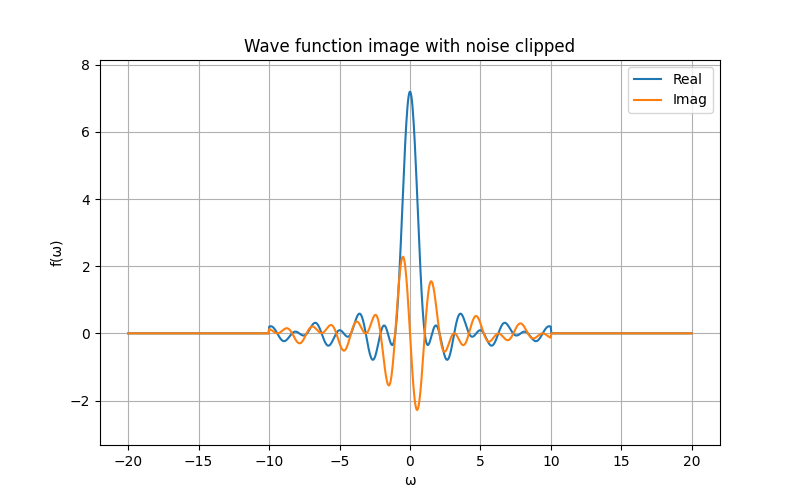
\includegraphics[width=\textwidth]{../results/\num/noised_wave_function_image_clipped.png}
%     \caption{Обрезанный образ функция $u(t)$ при $\omega_0=$~\imageclip}
%     \label{fig:noised_wave_function_image_clipped_\num}
% \end{figure}

\begin{figure}[ht!]
    \centering
    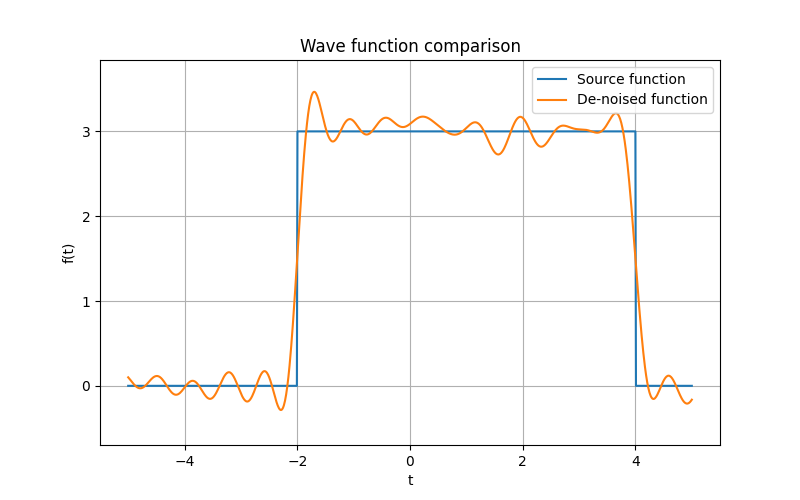
\includegraphics[width=\textwidth]{../results/\num/wave_function_comparison.png}
    \caption{Исходная и фильтрованная функция при $\omega_0=$~\imageclip}
    \label{fig:wave_function_comparison_\num}
\end{figure}

\FloatBarrier
Видим, что при уменьшении $\omega_0$ фильтрация становится более жесткой, что приводит к более сильному удалению шумов, но и к более сильному искажению самой функции.

\FloatBarrier
\subsubsection{Исследование влияния параметра b на фильтрацию}
Параметр $b$ влияет на амплитуду шумов в зашумленной функции. Таким образом, при его увеличении шумы становятся более заметными. 

\def\imageclip{10}
Рассмотрим несколько значений параметра $b$ при $\omega_0 =$~\imageclip~ и сравним результаты фильтрации.

\def\num{5}
\def\b{0.5}

\begin{figure}[ht!]
    \centering
    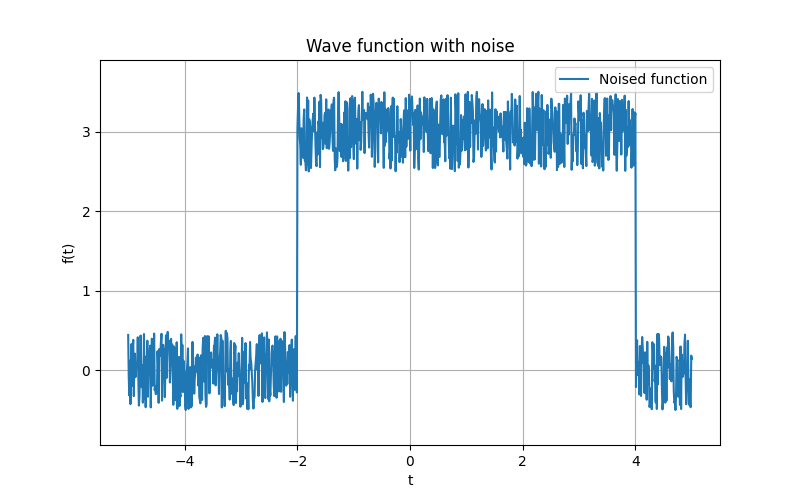
\includegraphics[width=\textwidth]{../results/\num/noised_wave_function.png}
    \caption{Функция $u(t)$ с параметрами $b = \b$, $c = \c$, $d = \d$}
    \label{fig:noised_wave_function_\num}
\end{figure}

\begin{figure}[ht!]
    \centering
    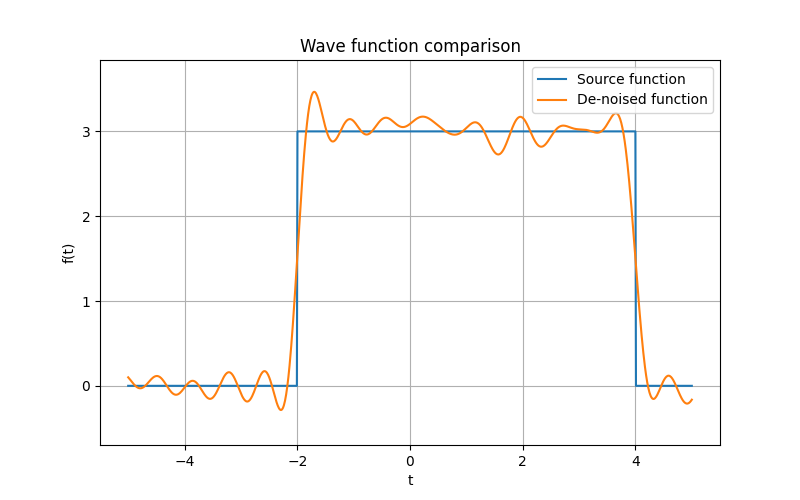
\includegraphics[width=\textwidth]{../results/\num/wave_function_comparison.png}
    \caption{Исходная и фильтрованная функция при $\omega_0=$~\imageclip}
    \label{fig:wave_function_comparison_\num}
\end{figure}


\def\num{6}
\def\b{2}

\begin{figure}[ht!]
    \centering
    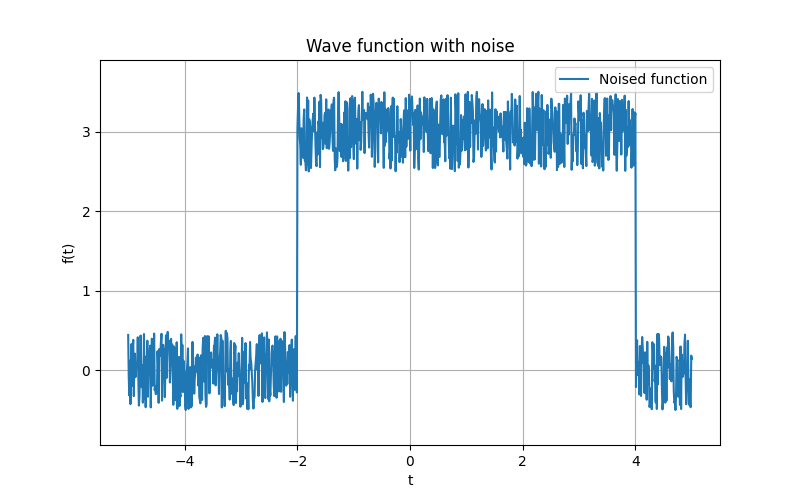
\includegraphics[width=\textwidth]{../results/\num/noised_wave_function.png}
    \caption{Функция $u(t)$ с параметрами $b = \b$, $c = \c$, $d = \d$}
    \label{fig:noised_wave_function_\num}
\end{figure}

\begin{figure}[ht!]
    \centering
    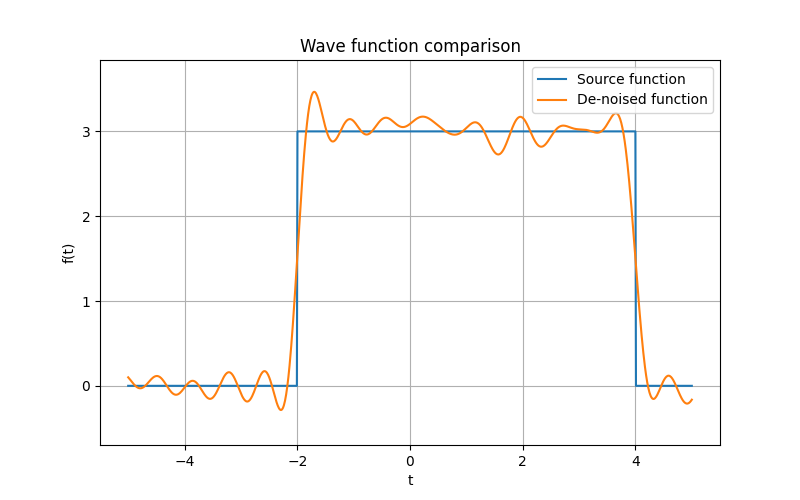
\includegraphics[width=\textwidth]{../results/\num/wave_function_comparison.png}
    \caption{Исходная и фильтрованная функция при $\omega_0=$~\imageclip}
    \label{fig:wave_function_comparison_\num}
\end{figure}


\def\num{7}
\def\b{0.2}

\begin{figure}[ht!]
    \centering
    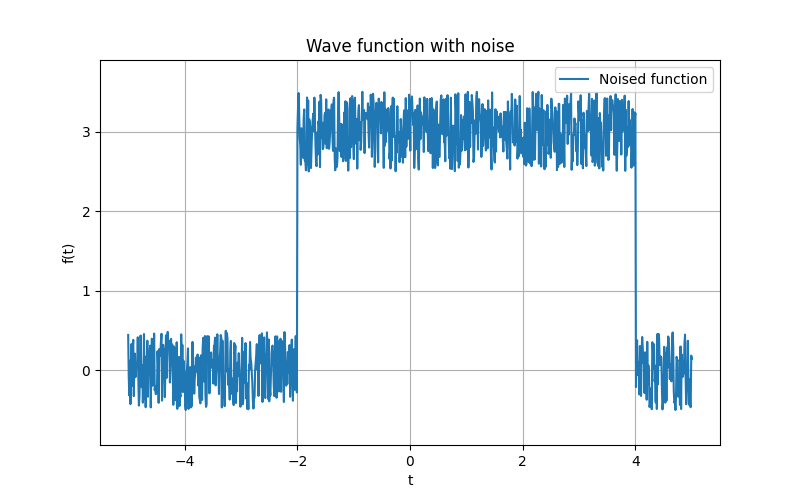
\includegraphics[width=\textwidth]{../results/\num/noised_wave_function.png}
    \caption{Функция $u(t)$ с параметрами $b = \b$, $c = \c$, $d = \d$}
    \label{fig:noised_wave_function_\num}
\end{figure}

\begin{figure}[ht!]
    \centering
    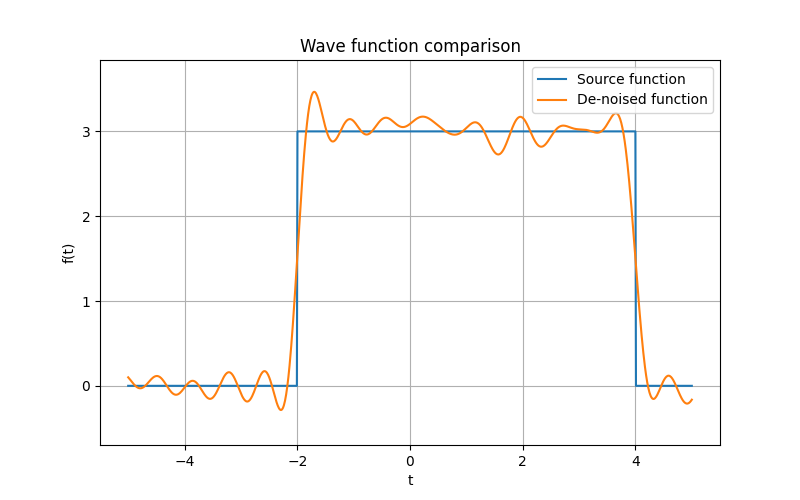
\includegraphics[width=\textwidth]{../results/\num/wave_function_comparison.png}
    \caption{Исходная и фильтрованная функция при $\omega_0=$~\imageclip}
    \label{fig:wave_function_comparison_\num}
\end{figure}

\def\num{8}
\def\b{4}

\begin{figure}[ht!]
    \centering
    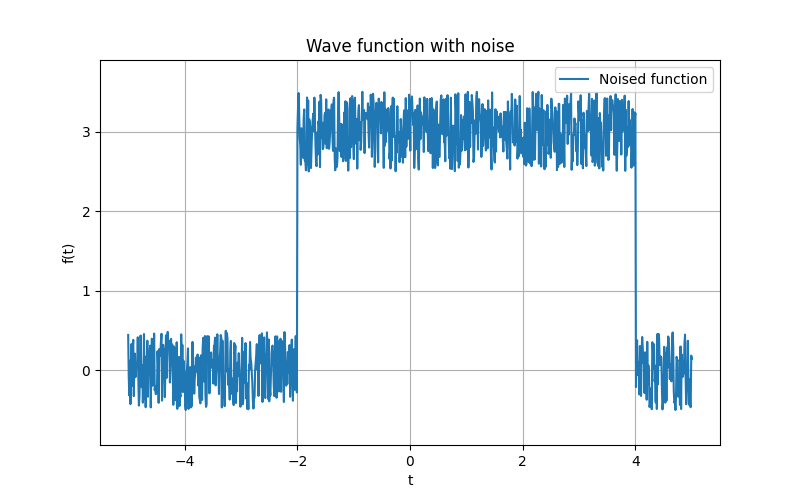
\includegraphics[width=\textwidth]{../results/\num/noised_wave_function.png}
    \caption{Функция $u(t)$ с параметрами $b = \b$, $c = \c$, $d = \d$}
    \label{fig:noised_wave_function_\num}
\end{figure}

\begin{figure}[ht!]
    \centering
    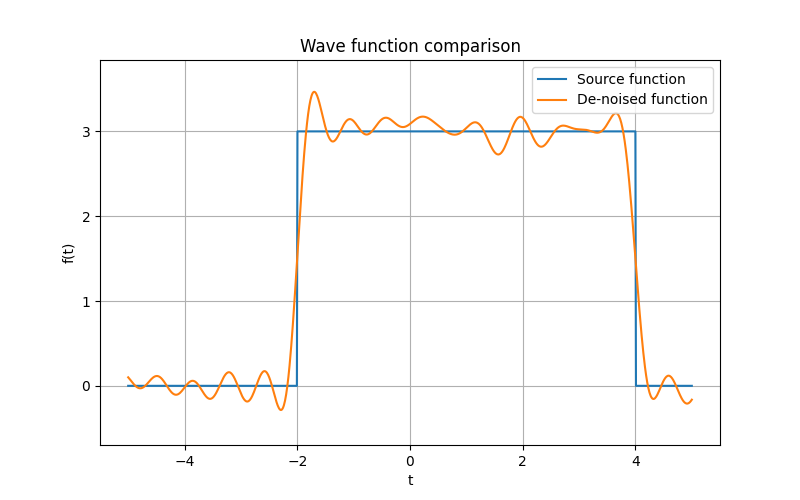
\includegraphics[width=\textwidth]{../results/\num/wave_function_comparison.png}
    \caption{Исходная и фильтрованная функция при $\omega_0=$~\imageclip}
    \label{fig:wave_function_comparison_\num}
\end{figure}

Видно, что при увеличении значения параметра $b$ шумы становятся более 
заметными, что приводит к более сильному искажению функции при фильтрации,
но даже при значении $b = 4$, когда исходная функция практически неразличима за шумом,
фильтрация все равно убирает шумы и восстанавливает функцию. Это связано с тем, что муш имеет 
только высокочастотные компоненты, которые удаляются при фильтрации.